\documentclass[a4paper,11pt]{article}

%% From https://github.com/aytchell/latex-listings-protobuf/tree/09c39676e6afb2af8c7d21ed21a516359c52e27c/

\usepackage{xcolor}
\usepackage{xcolor-solarized}
\usepackage{textcomp}

\newcommand{\SetProtoColorsSolarized}{
  % Colors taken from the 'solarized' color scheme of Ethan Schoonover
  % (with light background)
  % http://ethanschoonover.com/solarized
  \colorlet{proto_basic}{solarized-base00}
  \colorlet{proto_keyword}{solarized-cyan}
  \colorlet{proto_type}{solarized-cyan}
  \colorlet{proto_options}{solarized-cyan}
  \colorlet{proto_comment}{solarized-base1}
  \colorlet{proto_string}{solarized-blue}
  \colorlet{proto_number}{solarized-violet}
  \colorlet{proto_ident}{solarized-base00}
  \colorlet{proto_digits}{solarized-violet}
  \colorlet{proto_background}{solarized-base3}
}

\newcommand{\SetProtoColorsBlueish}{
  % Colors inspired by the NASM style of Robin Eklind
  % https://github.com/mewspring/latex
  \definecolor{proto_basic}{RGB}{0,0,0}             % black
  \definecolor{proto_keyword}{RGB}{0,0,0}         % black
  \definecolor{proto_ident}{RGB}{128,0,0}            % dark red
  \definecolor{proto_options}{RGB}{128,0,128}       % purple
  \definecolor{proto_comment}{RGB}{0,128,0}         % dark green
  \definecolor{proto_string}{RGB}{255,0,0}          % red
  \definecolor{proto_number}{RGB}{108,113,196}      % violet
  \definecolor{proto_type}{RGB}{0,0,255}             % blue
  \definecolor{proto_digits}{RGB}{0,0,128}          % dark blue
  \definecolor{proto_background}{RGB}{255,255,255}  % white
}

\newcommand{\SetProtoColorsTomorrow}{
  % Colors taken from the 'Tomorrow' color scheme of Chris Kempson
  % https://github.com/chriskempson/tomorrow-theme/blob/master/vim/colors/Tomorrow.vim
  \definecolor{proto_basic}{RGB}{77, 77, 76}          % dark grey
  %\definecolor{proto_keyword}{RGB}{245, 135, 31}      % orange
  \definecolor{proto_keyword}{RGB}{66, 113, 174}      % orange
  %\definecolor{proto_type}{RGB}{66, 113, 174}         % purple
  \definecolor{proto_type}{RGB}{200, 40, 41}         % red
  \definecolor{proto_options}{RGB}{137, 89, 168}
  %\definecolor{proto_comment}{RGB}{142, 144, 140}     % gray
  \definecolor{proto_comment}{RGB}{0,0,0}             % black
  \definecolor{proto_string}{RGB}{113, 140, 0}        % green
  \definecolor{proto_number}{RGB}{137, 89, 168}
  %\definecolor{proto_ident}{RGB}{200, 40, 41}         % red
  \definecolor{proto_ident}{RGB}{0,128,0}           % dark green
  \definecolor{proto_digits}{RGB}{245, 135, 31}       % orange
  \definecolor{proto_background}{RGB}{255, 255, 255}  % white
}

%\SetProtoColorsSolarized{}
\SetProtoColorsTomorrow{}
%\SetProtoColorsBlueish{}

\lstdefinestyle{protobuf}{
  frame=lines,
  %xleftmargin=\parindent,
  belowcaptionskip=1\baselineskip,
  backgroundcolor=\color{proto_background},
  basicstyle=\color{proto_basic}\footnotesize\ttfamily,
	keywordstyle=[1]\color{proto_keyword},
	keywordstyle=[2]\color{proto_type},
	keywordstyle=[3]\color{proto_options},
	commentstyle=\color{proto_comment},
	stringstyle=\color{proto_string},
  numberstyle=\color{proto_ident}\tiny,
  identifierstyle=\color{proto_ident}\bfseries,
	numbers=none, %left,
	numbersep=5pt,
	breaklines=false,
	showstringspaces=false,
	tabsize=2,
	prebreak=\raisebox{0ex}[0ex][0ex]{\ensuremath{\hookleftarrow}},
	upquote=true,
}


\usepackage{algorithm}
\usepackage{algpseudocode}
\usepackage{amsmath}
\usepackage{xcolor}
\usepackage{hyperref}
\usepackage{graphicx}

%\usepackage{sagetex}


\def\boxit#1{%
	\smash{\color{red}\fboxrule=1pt\relax\fboxsep=-2pt\llap{\rlap{\fbox{\strut\makebox[#1]{}}}~}}\ignorespaces
}

%\makeatletter
%\def\BState{\State\hskip-\ALG@thistlm}
%\makeatother

%opening
\title{zkInterface, a tool for zero-knowledge interoperability}
\author{Daniel Benarroch, Kobi Gurkan, Aurel Nicolas, Eran Tromer}

\begin{document}
	
	\maketitle
	
	%\begin{abstract}
		
	%\end{abstract}
	
	\section{Introduction}
	Implementing zero-knowledge proof constructions is not a trivial task and comes with diverse matters, as is extensively explained in the \href{https://zkproof.org/proceedings-snapshots/zkproof-implementation-20180801.pdf}{Implementation Track proceeding} of the first workshop. One of the requirements is to create a compiler of statements to be proven into a native low-level representation of the proving system.
	
	There are several trade-offs one can consider when designing general-purpose (front-end) compilers, lending to distinct frameworks, APIs, generality, etc. Today, existing compilers are implemented to work best with their corresponding (back-end) proving system (somemetimes more than one). For a comprehensive list of front-ends and back-ends, you can go to \href{https://zkp.science}{zkp.science}. 
	
	These libraries are usually built end-to-end: they take in some constraint system that defines the statement of the proving computation. In turn, there exist some tools to facilitate writing such constraint systems, which usually means compiling a program into R1CS, such as ZoKrates, gadget-lib or sapling-crypto.
	
	Generally, the compilers can output intermediary files and configurations, yet are used for a specific back-end. In practice this means there is no portability between proving systems and compilers. We aim to solve this issue by creating a community standard proposal for the ZKProof effort around constraint system formatting. We build upon the work done at the first ZKProof workshop, see the file format suggested and the further topics laid out. 
	
	In essence, we design and implement a standard rank-1 constraint system (R1CS) interface between front-ends and back-ends. Our design encompasses programmable instance and witness reductions, while capturing the underlying semantics, such as the scalar field or the depth of the merkle tree, among others.
	
	\paragraph{Background.} Zero-knowledge allow a prover to convince a verifier of the validity of some statement. In practice, these statements can be large and difficult to build, which is why developers usually build smaller components that are re-usable with different statements; these components are sometimes called ``gadgets". One can compose the different 
	
	
	\paragraph{Challenges}
	
	The main challenges of designing the interface come from the underlying semantics of the systems used. When compiling a given program into a constraint system, the different components have context to them
	
	- semantics
	- gadget composability
	- 
	
	\paragraph{Scope.} We aim for the standard interface to be as generic as possible, including non-R1CS-based proving systems. However, the current proposal is more limited, mainly due to time constraints.
	
	We propose to standardize the following:
	\begin{itemize}
		\item A file format for rank-1 constraint systems
		\item A messaging interface 
		\item A C API for interoperability
	\end{itemize}
	
	This proposal is not aiming to standardize a language or framework for generating constraint systems, nor the way that components of the proving statement should be written.  
	
	
	\paragraph{Motivation.} There is currently no other tool for combining zero knowledge front-ends to any back-end without creating a specific pair-wise interface. If you are a developer who has a favorite compiler to write constraints, with zkInterface, you can also chose your favorite implementation of any proving system. zkInterface can be seen as a common way to communicate between different zero-knowledge systems, as exemplified below.
	
	\begin{figure}[h!]
		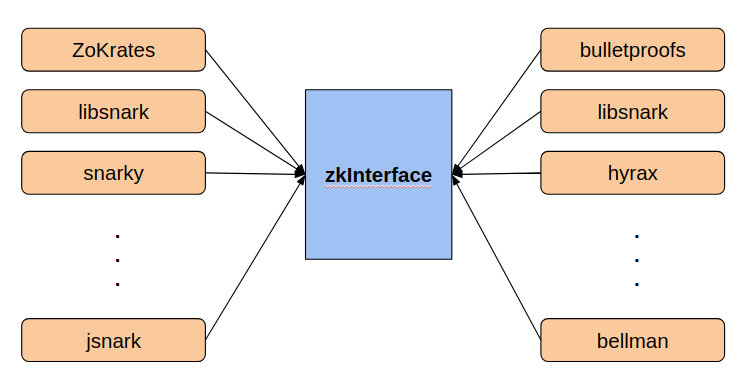
\includegraphics[width=\linewidth]{interface.png}
		\caption{zkInterface}
		\label{interface}
	\end{figure}
	
	
	\paragraph{Previous Work}
	
	The Implementation Track proceeding discusses some of the main issues that arise from the 
	
	
	
	
	\section{Description}
	
	zkInterface is a fully functional interface for zero-knowledge systems that enables an abstracted composition of components, by determining how data should be written and read. It can also be seen as a design tool for improved generation of constraints and usability, analogous to a portable binary format, since one can parametrize the functions calls and easily compose different functions, or components
	
	\paragraph{Terminology}
	The following list is in accordance to the terminology established in the 1st ZKProof Workshop.
	
	\begin{itemize}
		\item Parameter
		\item Argument
		\item Circuit
		\item Component (gadget)
		\item Script
		\item Witness
		\item Shared Inputs / Outputs
		\item Local Inputs / Outputs
		
	\end{itemize}
	
	\paragraph{Main functionality.}
	
	
	
		\begin{figure}[h!]
			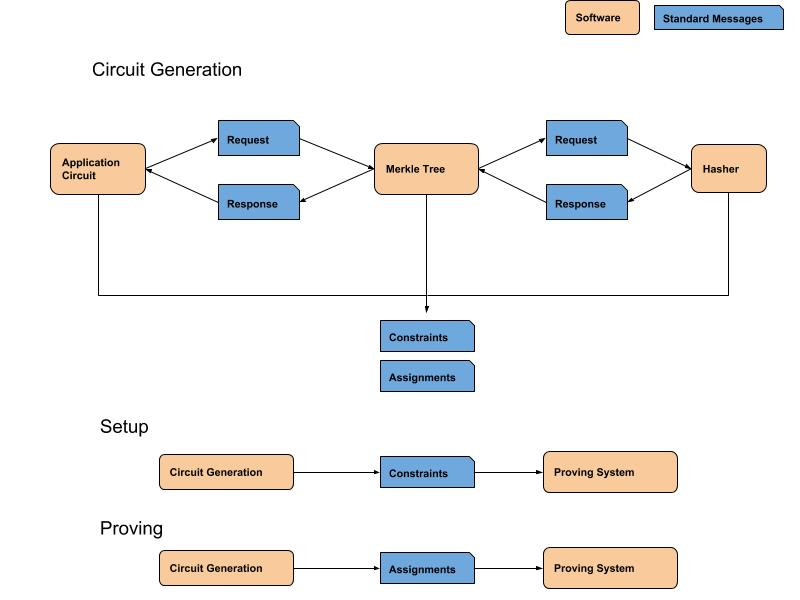
\includegraphics[width=\linewidth]{flow.jpg}
			\caption{The flow of interaction between existing libraries and the interface}
			\label{flow}
		\end{figure}
	
	\paragraph{Instance reduction.} 
	
	
	\paragraph{Witness reduction.}
	
	r1cs in the format: a way to represent the constraints and a way to represent the assignment; and connection between components (gadgets), which actually are the public inputs. If we think of circuit as components, each component has a set of local inputs and "outgoing" inputs.
	
	So the interface solves two problems: 1/ interop between frameworks (front-ends) and proving systems (backends) 2/ composability of gadgets between different frameworks.
	

	
	\subsection{An MVP}
	
	
	
	\subsection{Specification}
	
	*use of flatboard
	
	- semantics; planned parametrization of the semantics.
	
	- format: can work with files (all messages instead of processing, can be written to file) for both instance / witness reduction, otherwise can work with memory 
	
	Each component has an interface; which can be invoked / instantiated / called with other components to make up the constraint system.
		- composibility of gadgets as there local variables / public ones (merkle tree has the leaf and root and invokes sha256)
	
	CRS is specific to proving system so the format does not handle the CRS portability
	
	we are thinking of implementing ZoKrates for the application layer and libsnark, bellman.  
	
	NOTE: some people think of functions, inputs and returned variables; others as circuits and gadgets.
	
	
	Issues: 1/ linear 
\end{document}